\bookchapter{Chapitre 42 : Panorama des grands modèles et pratique de l'API}

\chapterintro{Les chapitres précédents portaient sur « comment collaborer avec l'IA » ; celui-ci répond à une question plus fondamentale : « quel IA choisir, et comment l'utiliser ? » Le paysage des grands modèles en août 2026 est d'une richesse extrême — à l'international, la rivalité des trois géants GPT, Claude et Gemini ; en Chine, une floraison de DeepSeek, Tongyi Qianwen, GLM, Kimi et Doubao. Chaque modèle a son tempérament et ses points forts : bien choisir, c'est un effort moitié moindre pour un résultat double ; mal choisir, l'inverse. Ce chapitre te présente ces modèles, t'apprend à les connecter à tes applications via une API et t'aide à choisir le Token Plan (forfait d'usage) adapté à tes besoins.}

\booksection{Les grands modèles internationaux : un trio de tête}

En août 2026, le marché international des grands modèles s'organise autour d'un trio : OpenAI (série GPT), Anthropic (série Claude) et Google (série Gemini). Chacun a une identité bien marquée — faisons connaissance un par un.

\booksubsection{La série OpenAI GPT-5.6 : le généraliste au profil sans faille}

OpenAI a déclenché la vague des grands modèles, et la série GPT demeure le plus utilisé des modèles au monde. Publiée en juillet 2026, la série GPT-5.6 adopte une stratégie en trois gammes : le vaisseau amiral GPT-5.6 Sol vise le raisonnement haut de gamme, le modèle équilibré GPT-5.6 Terra vise le développement quotidien, et le modèle léger GPT-5.6 Luna vise les scénarios à fort trafic et faible coût. Les trois partagent une fenêtre de contexte de 1,05 million de Token et acceptent tous les entrées image, les appels de fonctions et les sorties structurées.

\begin{center}
\begin{tabularx}{\linewidth}{|X|X|X|X|X|}
\hline
\textbf{Modèle} & \textbf{Positionnement} & \textbf{Entrée (/million de Token)} & \textbf{Sortie (/million de Token)} & \textbf{Fenêtre de contexte} \tabularnewline
\hline
GPT-5.6 Sol & Raisonnement haut de gamme & 5,00 US\$ (environ 36 yuans) & 30,00 US\$ (environ 217 yuans) & 1,05 M Token \tabularnewline
GPT-5.6 Terra & Polyvalent quotidien & 2,50 US\$ (environ 18 yuans) & 15,00 US\$ (environ 109 yuans) & 1,05 M Token \tabularnewline
GPT-5.6 Luna & Léger et économique & 1,00 US\$ (environ 7 yuans) & 6,00 US\$ (environ 44 yuans) & 1,05 M Token \tabularnewline
\hline
\end{tabularx}
\end{center}

\begin{center}\small\color{gray}Tarifs de la série OpenAI GPT-5.6 (août 2026)\end{center}

L'atout majeur de la série GPT, c'est son équilibre — raisonnement, code, écriture, multimodal : aucun point faible marqué. Ajoute l'immense écosystème de plugins et la communauté de développeurs d'OpenAI : la documentation et la chaîne d'outils sont les plus complètes du marché. Pour les cas où « on ne sait pas quoi choisir », GPT est la réponse par défaut, celle qu'on peut choisir les yeux fermés. Ses faiblesses : l'accès depuis la Chine exige un réseau particulier, l'expression chinoise sonne parfois « traduite », et le prix de l'API se situe dans le haut du panier.

\textbf{Bonne nouvelle}\par

En août 2026, OpenAI a annoncé que le modèle par défaut des utilisateurs gratuits passait à GPT-5.6 Luna, avec discussion texte illimitée. Concrètement, tu peux découvrir les capacités de base de GPT à coût zéro ; tu ne paies que si tu as besoin d'un raisonnement plus puissant ou d'appels API.

\booksubsection{La série Anthropic Claude : le sommet du code et de la rigueur}

Si GPT est le polyvalent, Claude est le « sommet » du domaine de la programmation. La série Claude d'Anthropic domine depuis longtemps, avec une avance écrasante, le SWE-bench (benchmark d'ingénierie logicielle) : première du secteur pour la qualité de génération de code et la capacité à mener des projets de niveau ingénierie. Détail précieux : le taux d'hallucination de Claude (probabilité de produire de fausses informations) est le plus bas du marché, environ 1 \% — parfait pour les scénarios de haute précision comme la recherche ou le juridique.

L'autre arme secrète de Claude est son très long contexte : une fenêtre de 1 million de Token, capable d'« avaler » d'un coup des centaines de pages de contrat ou une bibliothèque de code entière sans perdre un détail. Presque irremplaçable pour le refactoring de code ou l'analyse de longs documents. Claude Code, l'outil de programmation IA en terminal, atteignait mi-2026 un revenu annualisé de 2,5 milliards de dollars — la meilleure preuve de la reconnaissance des talents de Claude en programmation.

\begin{center}
\begin{tabularx}{\linewidth}{|X|X|X|X|X|}
\hline
\textbf{Modèle} & \textbf{Positionnement} & \textbf{Entrée (/million de Token)} & \textbf{Sortie (/million de Token)} & \textbf{Fenêtre de contexte} \tabularnewline
\hline
Claude Fable 5 & Vaisseau amiral & 10,00 US\$ (environ 72 yuans) & 50,00 US\$ (environ 362 yuans) & 1 M Token \tabularnewline
Claude Opus 4.8 & Modèle Pro & 5,00 US\$ (environ 36 yuans) & 25,00 US\$ (environ 181 yuans) & 1 M Token \tabularnewline
Claude Sonnet 5 & Rapport qualité-prix & 2,00 US\$ (environ 14 yuans) & 10,00 US\$ (environ 72 yuans) & 1 M Token \tabularnewline
\hline
\end{tabularx}
\end{center}

\begin{center}\small\color{gray}Tarifs de la série Anthropic Claude (août 2026 ; Sonnet 5 au prix promotionnel)\end{center}

La faiblesse de Claude, c'est le prix : la sortie de Fable 5 est la plus chère de tous les modèles, 50 dollars par million de Token. Ses capacités multimodales (compréhension des images et des vidéos) restent aussi relativement modestes. Pour le développeur individuel au budget serré, Sonnet 5 en période promotionnelle offre un rapport qualité-prix remarquable.

\booksubsection{La série Google Gemini : le roi du multimodal}

La série Gemini de Google en est, en 2026, à la version 3.1 Pro. Son atout majeur est le multimodal natif : analyse texte-image d'une grande précision, reconnaissance OCR des tableaux sans erreur, extraction efficace des images vidéo, sans oublier l'analyse poussée de l'audio et de la vidéo. Profondément lié à l'écosystème Google (recherche, messagerie, services cloud), il brille dans la recherche d'informations en temps réel et la compréhension intermodale. Gemini accepte aussi une entrée de contexte de 2 millions de Token — la plus grande fenêtre de contexte du moment.

Gemini se positionne comme « le premier choix pour le raisonnement scientifique et les scénarios multimodaux ». Si ton projet implique beaucoup d'analyse d'images, de compréhension vidéo ou de calcul scientifique, Gemini n'a presque aucun rival. Mais il est légèrement en retrait de Claude pour la génération de code en texte pur, et son chinois est moins naturel que celui des modèles chinois.

\begin{center}
\begin{tabularx}{\linewidth}{|X|X|X|X|}
\hline
\textbf{Critère} & \textbf{GPT-5.6} & \textbf{Claude Fable 5} & \textbf{Gemini 3.1 Pro} \tabularnewline
\hline
Score global & 94.8 & 95.0 & 92.1 \tabularnewline
Capacité de code (SWE-bench) & 74.9\% & 64.3\% (Pro) & Moyen \tabularnewline
Fenêtre de contexte & 1,05 M Token & 1 M Token & 2 M Token \tabularnewline
Capacités multimodales & Équilibré & Faibles & Le plus fort \tabularnewline
Taux d'hallucination & Plutôt bas & Le plus bas (environ 1 \%) & Plutôt bas \tabularnewline
Accessibilité depuis la Chine & Réseau particulier requis & Réseau particulier requis & Réseau particulier requis \tabularnewline
Écosystème API & Le plus complet & En croissance & Lié à l'écosystème Google \tabularnewline
\hline
\end{tabularx}
\end{center}

\begin{center}\small\color{gray}Comparaison des trois grands modèles internationaux (août 2026)\end{center}

\begin{tcbwarn}{Attention : l'obstacle concret de l'usage en Chine}
Pour les développeurs en Chine, le principal obstacle à GPT, Claude et Gemini est l'accès réseau. On peut passer par des relais Azure ou des plateformes d'agrégation d'API, mais la stabilité et la conformité restent à évaluer soi-même. Si ton projet impose des exigences strictes de sécurité des données, commence par regarder les modèles chinois.

\end{tcbwarn}

\booksection{Les grands modèles chinois : une floraison d'acteurs}

En 2026, les grands modèles chinois ne sont plus des « poursuivants » mais des « coureurs au coude à coude », voire des « meneurs » dans certains domaines. Contrairement aux polémiques sur les « coquilles » (wrappers) de 2023, les modèles chinois phares de 2026 rivalisent avec les meilleurs modèles internationaux en raisonnement logique, génération de code et compréhension du chinois, l'écart s'étant réduit sous les 5 \%. Mieux : les modèles chinois possèdent des atouts irremplaçables en scénarios chinois, en coût et en déploiement conforme.

\booksubsection{DeepSeek V4 : le roi du rapport qualité-prix}

DeepSeek est un phénomène parmi les grands modèles chinois. Début 2025, DeepSeek-V3 a secoué le marché avec son positionnement « dix fois moins cher que GPT pour une capacité équivalente », au point que le milieu parle de sa « ligne d'élimination de l'IA générale » : moins cher que lui, c'est moins bon ; plus cher, rien ne délivre autant de volume. En août 2026 est sortie la version officielle de DeepSeek V4-Pro : architecture MoE de 1,6 billion de paramètres avec environ 49B activés, contexte sans perte d'1 million de Token — son rapport qualité-prix en code est largement considéré comme le plafond mondial.

DeepSeek V4 a fait un bond considérable en capacités d'Agent : le benchmark DeepSWE est passé de 12,8 à 62,7 (+390 \%) et NL2Repo de 38,5 à 61,5. Son API ajoute la prise en charge du double protocole Responses API et Anthropic API, qui le rend compatible avec les grands outils de programmation comme Codex et Claude Code. Autrement dit, tu peux remplacer l'API de Claude par celle de DeepSeek dans Claude Code — pour un coût divisé plusieurs fois, avec une expérience presque identique.

\begin{center}
\begin{tabularx}{\linewidth}{|X|X|X|X|X|}
\hline
\textbf{Modèle} & \textbf{Positionnement} & \textbf{Entrée (/million de Token)} & \textbf{Sortie (/million de Token)} & \textbf{Fenêtre de contexte} \tabularnewline
\hline
DeepSeek V4 Pro & Raisonnement haut de gamme & 3 yuans (environ 0,43 US\$) & 6 yuans (environ 0,87 US\$) & 1 M Token \tabularnewline
DeepSeek V4 Flash & Léger et rapide & 1 yuan (environ 0,14 US\$) & 2 yuans (environ 0,28 US\$) & 1 M Token \tabularnewline
\hline
\end{tabularx}
\end{center}

\begin{center}\small\color{gray}Tarifs de la série DeepSeek V4 (août 2026, prix promotionnels)\end{center}

Comparaison de prix : pour le même lot d'1 million de Token en entrée + 1 million de Token en sortie, DeepSeek V4 Flash coûte environ 0,42 dollar, GPT-5.6 Sol environ 35 dollars et Claude Fable 5 environ 60 dollars. Un écart pouvant atteindre 80 à 140 fois.

\textbf{Alerte piège : DeepSeek va augmenter ses prix}\par

DeepSeek a officiellement annoncé le 6 août 2026 son « intention d'augmenter fortement ses tarifs API prochainement » : le prix promotionnel pourrait ne pas durer. Certains médias évoquent une hausse pouvant aller jusqu'à 30 fois ; au 14 août, la grille finale n'était pas encore publiée. Par ailleurs, la version officielle de DeepSeek V4 introduit une tarification heures pleines/heures creuses : en heure de pointe, le prix d'appel double carrément. Surveille les annonces officielles pour les tarifs à jour.

\booksubsection{Qwen3.7 Max de Tongyi Qianwen : le choix entreprise d'Alibaba Cloud}

La série Qwen (Tongyi Qianwen) d'Alibaba Cloud s'appuie sur son écosystème cloud et dispose d'atouts naturels pour le déploiement en entreprise. Qwen3.7 Max, sorti en juillet 2026, est le vaisseau amiral actuel : modèle dense de 235B paramètres, contexte natif de 256K extensible à 1M. Les forces clés de Qwen : un écosystème open source mûr (toute la gamme, de 7B à 235B, est ouverte), une compréhension fine des scénarios chinois et une intégration profonde avec l'infrastructure d'Alibaba Cloud.

\begin{center}
\begin{tabularx}{\linewidth}{|X|X|X|}
\hline
\textbf{Modèle} & \textbf{Prix de sortie (/million de Token)} & \textbf{Cas d'usage} \tabularnewline
\hline
qwen-turbo & 0,6 yuan & Q\&R minimaliste, classification de texte, fort trafic \tabularnewline
qwen-long & 2,0 yuans & Traitement de très longs contextes (10M) \tabularnewline
qwen3.7-flash & 7,2 yuans & Conversation générale, génération de contenu \tabularnewline
qwen3.7-plus & 12,0 yuans & Multimodal (images + vidéos), création en chinois \tabularnewline
qwen3.7-max & 36,0 yuans & Capacités chinoises phares, tâches complexes \tabularnewline
\hline
\end{tabularx}
\end{center}

\begin{center}\small\color{gray}Tarification par paliers de la série Qwen de Tongyi Qianwen (août 2026)\end{center}

Qwen pratique une tarification par paliers — du très économique qwen-turbo (sortie à 0,6 yuan/million de Token) au vaisseau amiral qwen3.7-max (sortie à 36 yuans/million de Token), couvrant tous les besoins, de la simple Q\&R au raisonnement complexe. Pour les entreprises déjà sur Alibaba Cloud, Qwen est l'option d'intégration la plus naturelle.

\booksubsection{GLM-5.1 de Zhipu : premier chinois au SWE-bench}

La série GLM de Zhipu AI brille en 2026. GLM-5.1 décroche la première place chinoise au SWE-bench : architecture hybride dense MoE de 744B, contexte d'1 million de Token. Il se distingue par une compréhension sémantique du chinois très précise et un déploiement privé conforme aux règles chinoises — essentiel pour la finance et l'administration, très exigeantes en sécurité des données. GLM-5.1 est facturé 6 yuans en entrée et 24 yuans en sortie par million de Token, soit le milieu du panier chinois.

\booksubsection{Kimi K3 : le roi du très long texte}

La série Kimi de Moonshot AI est célèbre pour son traitement des très longs textes. Kimi K3, publié en juillet 2026, affiche 2,8 billions de paramètres et rejoint le premier peloton mondial sur de nombreux tests de tâches complexes. Le cœur de Kimi : l'analyse de longues bases de code et la recherche augmentée dans de longs documents — il avale le texte d'un livre entier ou le code d'un projet complet, et excelle dans les tâches de recherche de type « aiguille dans une botte de foin ». Sa tarification est relativement élevée (sortie d'environ 12 à 20 yuans/million de Token), mais son rapport qualité-prix sur les longs textes reste imbattable.

\booksubsection{Doubao : le polyvalent de ByteDance}

La série Doubao de ByteDance est d'une belle régularité en 2026. Doubao Seed 2.1 Pro est le modèle phare de Volcano Engine : 256K de contexte, une performance globale stable en tests réels et une expérience remarquable en chinois. Ses atouts : une grosse dotation de Token gratuits dès l'inscription, une intégration complète à l'écosystème Volcano Engine et des tarifs parmi les plus bas de Chine. Pour le débutant qui veut goûter vite à la programmation IA, Doubao est la porte d'entrée sans barrière.

\begin{center}
\begin{tabularx}{\linewidth}{|X|X|X|X|X|X|}
\hline
\textbf{Critère} & \textbf{DeepSeek V4} & \textbf{Qwen3.7 Max} & \textbf{GLM-5.1} & \textbf{Kimi K3} & \textbf{Doubao 2.1 Pro} \tabularnewline
\hline
Score global & 87.5 & 89.7 & 90.5 & 88+ & 85+ \tabularnewline
Capacité de code & Très fort & Fort & Premier chinois au SWE & Fort & Au-dessus de la moyenne \tabularnewline
Compréhension du chinois & Excellent & Excellent & Précis & Excellent & Excellent \tabularnewline
Fenêtre de contexte & 1 M & 256K-1M & 1 M & Très long & 256K \tabularnewline
Prix de sortie (yuans/M) & 6 & 36 & 24 & 12-20 & 30 \tabularnewline
Open source & Licence MIT & Toute la gamme ouverte & Partiellement ouvert & Fermé & Fermé \tabularnewline
Déploiement privé & Oui & Oui & Oui & Non & Non \tabularnewline
\hline
\end{tabularx}
\end{center}

\begin{center}\small\color{gray}Comparaison des cinq grands modèles chinois (août 2026)\end{center}

Une tendance importante : le « sentiment d'écart de génération » entre modèles chinois et GPT/Claude a disparu. En raisonnement logique comme en compétition mathématique, l'écart entre les modèles chinois phares et GPT-5 se compte en unités. Sur la pensée d'architecture systémique et le raisonnement d'ingénierie complexe, Claude garde l'avantage — ses propositions d'architecture ont plus d'« inspiration », quand les modèles chinois paraissent parfois « dogmatiques ». Mais sur les scénarios chinois, la maîtrise des coûts et le déploiement conforme, les modèles chinois ont une avance écrasante.

\begin{center}
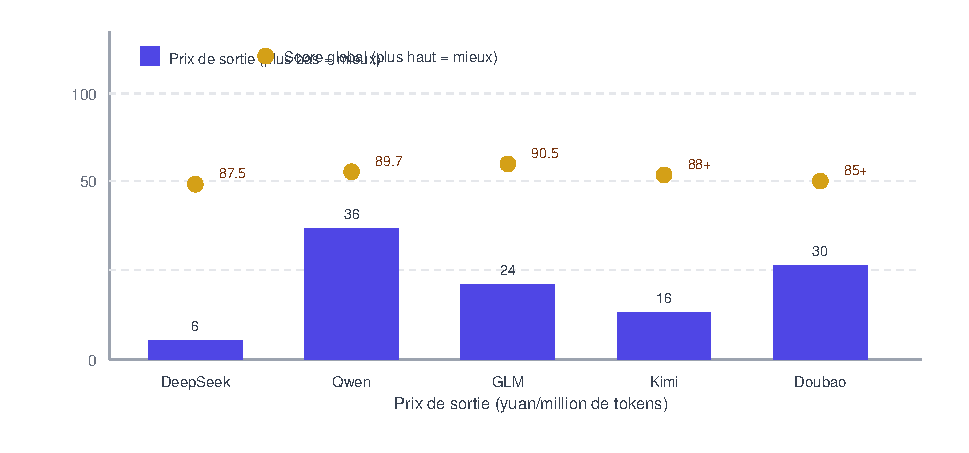
\includegraphics[width=0.92\linewidth]{figures/fig-di-si-shi-er-zhang-1}
\\[2pt]\small Figure 4 : prix et performance des cinq modèles (prix le plus bas possible, score le plus haut possible)
\end{center}

\booksection{Le cadre de décision pour choisir un modèle}

Une fois les caractéristiques de chaque modèle en tête, comment choisir pour ton projet ? Voici la « méthode des quatre questions » : y répondre suffit à verrouiller le modèle le plus adapté.

Ton projet est-il déployé en Chine ou à l'international ?

En Chine choisis des modèles nationaux

|

International modèles étrangers possibles

La tâche principale est-elle de coder ou autre chose ?

Coder Claude ou DeepSeek

|

Autre chose continue l'évaluation

Besoin d'un contexte très long (>500 000 tokens) ?

Oui Gemini ou Kimi

|

Pas besoin continue l'évaluation

Budget serré ?

Serré DeepSeek ou Qwen-turbo

|

Peu sensible GPT-5.6 ou Claude

\begin{center}\small\color{gray}Figure 5 : la méthode des quatre questions pour choisir un grand modèle\end{center}

\begin{tcbinfo}{Astuce : la stratégie de combinaison}
Cette méthode n'est pas un dogme — beaucoup de scénarios demandent de combiner plusieurs modèles. Une combinaison courante : DeepSeek ou Qwen pour le développement quotidien (coût bas, bon en chinois), Claude pour les décisions d'architecture critiques (raisonnement puissant, peu d'hallucinations), Gemini pour l'analyse multimodale (traitement des images et vidéos). Change de modèle selon le besoin, au lieu de « faire vivre un seul modèle jusqu'au bout ».

\end{tcbinfo}

\booksection{Premiers pas avec l'API : brancher un grand modèle à partir de zéro}

Beaucoup de tutos de programmation IA se limitent à l'interface de discussion, mais la vraie « programmation IA » — faire appeler un grand modèle par ton application — passe par une API. Une API (Application Programming Interface) est un protocole de communication entre programmes. Via l'API, ton code peut mobiliser la puissance d'un grand modèle comme s'il appelait une simple fonction.

\booksubsection{Qu'est-ce qu'un Token}

Avant d'aborder l'API, il faut comprendre la notion de « Token ». Le Token est l'unité de facturation de base des grands modèles — l'« unité de lecture et d'écriture de l'IA ». Un Token correspond environ à 0,75 mot anglais (4 caractères) ou à 0,5 à 1 caractère chinois. Un texte chinois de 1000 caractères consomme à peu près 1500 à 2000 Token.

Un Token n'est ni un mot ni un caractère. Les grands modèles découpent le texte en Token grâce à un tokenizer dédié. Le même mot peut donner un nombre différent de Token selon le modèle — un même terme peut ainsi valoir 3 Token dans GPT et 2 dans DeepSeek. La plupart des API renvoient le nombre de Token réellement consommé : tu peux le vérifier dans la réponse de l'API.

\begin{tcbinfo}{Estimation rapide du coût en Token}
Un million de caractères chinois équivaut à environ 1,5 million de Token. Traiter 1 million de caractères en entrée + 1 million en sortie avec DeepSeek V4 Flash coûte environ 0,42 dollar (environ 3 yuans) ; avec Claude Fable 5, le même volume coûte environ 60 dollars (environ 434 yuans). Voilà pourquoi le choix du modèle pèse directement sur le coût de ton projet.

\end{tcbinfo}

\booksubsection{Obtenir une clé API}

La première étape pour utiliser l'API d'un grand modèle est d'obtenir une clé API — une chaîne secrète servant à l'authentification. Chaque fournisseur de modèles a sa propre plateforme API : crée un compte puis génère ta clé API. Voici les portails API des modèles principaux et la marche à suivre :

\begin{center}
\begin{tabularx}{\linewidth}{|X|X|X|X|}
\hline
\textbf{Modèle} & \textbf{Plateforme API} & \textbf{Démarche d'obtention} & \textbf{Quota gratuit} \tabularnewline
\hline
DeepSeek & platform.deepseek.com & Inscription vérification d'identité création de la clé API & Quota offert aux nouveaux comptes \tabularnewline
Tongyi Qianwen & bailian.aliyun.com (plateforme Bailian) & Connexion au compte Alibaba Cloud activation du service création de la clé & Essai gratuit pour nouveaux comptes \tabularnewline
Zhipu GLM & open.bigmodel.cn & Inscription vérification d'identité création de la clé API & Quota offert aux nouveaux comptes \tabularnewline
Kimi & platform.moonshot.cn & Inscription vérification d'identité création de la clé API & Quota gratuit limité \tabularnewline
Doubao & volcengine.com (Volcano Engine) & Inscription activation d'Ark création de la clé API & Beaucoup de Token offerts à l'inscription \tabularnewline
OpenAI GPT & platform.openai.com & Inscription carte bancaire rattachée création de la clé API & Pas de quota gratuit (payant) \tabularnewline
Anthropic Claude & console.anthropic.com & Inscription carte rattachée création de la clé API & Petit quota pour nouveaux comptes \tabularnewline
\hline
\end{tabularx}
\end{center}

\begin{center}\small\color{gray}Plateformes API des grands modèles et obtention des clés (août 2026)\end{center}

\textbf{Conseil sécurité : ta clé API = le mot de passe de ton portefeuille}\par

La clé API vaut le mot de passe de ton portefeuille — quiconque la détient peut consommer ton quota. Donc : n'écris jamais une clé API dans le code (gère-la par variables d'environnement) ; ne pousse jamais de code contenant la clé vers un dépôt Git public ; ne partage jamais de capture d'écran où elle apparaît. Si la clé fuit, supprime-la immédiatement sur la plateforme et recrée-en une.

\booksubsection{Ton premier appel d'API}

Une fois la clé API en main, tu peux appeler l'API d'un grand modèle dans n'importe quel langage de programmation. Voici en Python l'appel le plus simple — envoyer un message à DeepSeek et récupérer sa réponse.

\begin{lstlisting}[language=Python]
# Installe le SDK : pip install openai
# DeepSeek est compatible avec le SDK OpenAI, utilisable directement
from openai import OpenAI
import os

# 1. créer le client (la clé API se lit dans la variable d'environnement)
client = OpenAI(
    api_key=os.environ.get("DEEPSEEK_API_KEY"),
    base_url="https://api.deepseek.com"
)

# 2. envoyer la requête
response = client.chat.completions.create(
    model="deepseek-chat",  # modèle choisi
    messages=[
        {"role": "system", "content": "Tu es un assistant de programmation Python."},
        {"role": "user", "content": "Écris une fonction de tri rapide."}
    ]
)

# 3. récupérer la réponse
print(response.choices[0].message.content)

# 4. voir la consommation de tokens
print(f"Tokens d'entrée : {response.usage.prompt_tokens}")
print(f"Tokens de sortie : {response.usage.completion_tokens}")
print(f"Tokens totaux : {response.usage.total_tokens}")
\end{lstlisting}

La logique de ce code : créer le client (avec la clé API et l'adresse du modèle) construire la liste des messages (system définit le rôle, user porte la saisie de l'utilisateur) envoyer la requête récupérer la réponse. Ce schéma vaut pour presque tous les modèles compatibles avec le format OpenAI : changer de modèle revient à remplacer api\_key et base\_url. C'est pourquoi tant de modèles chinois choisissent la compatibilité avec le SDK OpenAI : deux lignes de code suffisent pour changer de modèle, à un coût de migration minime.

Voici les différences de code pour passer à un autre modèle — remarque qu'il suffit de changer deux lignes :

\begin{lstlisting}[language=Python]
# DeepSeek
client = OpenAI(
    api_key=os.environ.get("DEEPSEEK_API_KEY"),
    base_url="https://api.deepseek.com"
)
# model="deepseek-chat"

# Qwen (plateforme Bailian)
client = OpenAI(
    api_key=os.environ.get("DASHSCOPE_API_KEY"),
    base_url="https://dashscope.aliyuncs.com/compatible-mode/v1"
)
# model="qwen-plus"

# GLM de Zhipu
client = OpenAI(
    api_key=os.environ.get("GLM_API_KEY"),
    base_url="https://open.bigmodel.cn/api/paas/v4"
)
# model="glm-4"

# OpenAI GPT
client = OpenAI(
    api_key=os.environ.get("OPENAI_API_KEY"),
    # le base_url par défaut suffit
)
# model="gpt-5.6-terra"
\end{lstlisting}

\booksubsection{Traiter les réponses en flux}

En pratique, tu ne veux généralement pas attendre que l'IA ait tout écrit avant d'afficher d'un bloc — l'utilisateur attendrait trop. La réponse en flux (streaming) affiche le texte mot à mot pendant que l'IA génère, ce qui améliore nettement l'expérience : comme sur une machine à écrire, les caractères jaillissent un à un, et la sensation est tout autre.

\begin{lstlisting}[language=Python]
# Réponse en streaming : sortie mot à mot
stream = client.chat.completions.create(
    model="deepseek-chat",
    messages=[
        {"role": "user", "content": "Écris un tutoriel du tri à bulles en Python"}
    ],
    stream=True  # active le streaming
)

# reçoit et affiche par blocs
for chunk in stream:
    if chunk.choices[0].delta.content is not None:
        print(chunk.choices[0].delta.content, end="", flush=True)
# la sortie s'affichera lettre par lettre, comme une machine à écrire
\end{lstlisting}

\booksection{Guide d'achat des Token Plan}

La plupart des fournisseurs proposent deux modes de facturation : le paiement à l'usage (Pay-as-you-go) et l'abonnement par forfait (Token Plan / Subscription). Comprendre la différence t'aidera à réduire nettement tes coûts d'usage.

\booksubsection{Paiement à l'usage vs abonnement}

\begin{center}
\begin{tabularx}{\linewidth}{|X|X|X|}
\hline
\textbf{Dimension} & \textbf{Paiement à l'usage (Pay-as-you-go)} & \textbf{Abonnement (Subscription)} \tabularnewline
\hline
Mode de facturation & Tu paies les Token que tu consommes & Somme fixe payée d'avance contre un quota \tabularnewline
Cas d'usage & Usage irrégulier, appels occasionnels & Usage régulier, appels fréquents \tabularnewline
Avantage de prix & Prix standard & 20 \% à 50 \% moins cher qu'à l'usage \tabularnewline
Souplesse & Disponible à tout moment, sans engagement & Prépaiement requis, le quota peut expirer \tabularnewline
Dépassement de quota & Facturation à l'usage automatique & Basculer à l'usage une fois le quota dépassé \tabularnewline
Plateformes types & Les plateformes API officielles de chaque modèle & OpenAI Plus/Pro, Claude Pro, Cursor Pro \tabularnewline
\hline
\end{tabularx}
\end{center}

\begin{center}\small\color{gray}Comparaison des deux modes de facturation\end{center}

Pour débuter, commence par le paiement à l'usage — aucun prépaiement, tu ne dépenses que ce que tu consommes. Quand ton volume mensuel se stabilise (par exemple au-delà de 50 yuans par mois), envisage de passer à l'abonnement pour un prix unitaire plus bas.

\booksubsection{Tour d'horizon des abonnements principaux}

\begin{center}
\begin{tabularx}{\linewidth}{|X|X|X|X|}
\hline
\textbf{Forfait} & \textbf{Tarif mensuel} & \textbf{Contenu inclus} & \textbf{Pour qui} \tabularnewline
\hline
ChatGPT Free & Gratuit & Conversations texte illimitées avec GPT-5.6 Luna & Découverte sans prérequis \tabularnewline
ChatGPT Plus & 20 US\$/mois & GPT-5.6 Sol, génération d'images, analyse de données, accès aux plugins & Utilisateurs réguliers \tabularnewline
ChatGPT Pro & 200 US\$/mois & Tous les modèles sans limite, accès prioritaire aux nouveautés & Professionnels intensifs \tabularnewline
Claude Free & Gratuit & Nombre limité de conversations Claude & Découverte sans prérequis \tabularnewline
Claude Pro & 20 US\$/mois & Claude sans limite, accès prioritaire aux nouveaux modèles & Développeurs \tabularnewline
Cursor Free & Gratuit & Complétions IA et conversations en nombre limité & Essai pour débutants \tabularnewline
Cursor Pro & 20 US\$/mois & Complétion IA illimitée, 500 requêtes avancées/mois & Développeurs du quotidien \tabularnewline
Cursor Business & 40 US\$/mois/personne & Collaboration d'équipe, console d'administration, mode confidentialité & Usage en équipe \tabularnewline
\hline
\end{tabularx}
\end{center}

\begin{center}\small\color{gray}Abonnements des principaux outils IA (août 2026)\end{center}

Les formules des modèles chinois diffèrent un peu. DeepSeek fonctionne surtout à l'usage, sans abonnement mensuel — tu recharges ton compte et tu paies selon ta consommation réelle. Tongyi Qianwen propose sur la plateforme Bailian des packs prépayés (tu achètes un quota de Token à prix réduit). Doubao offre des formules prépayées similaires sur Volcano Engine. Pour un développeur en Chine, la combinaison la plus économique est généralement : DeepSeek à l'usage (développement quotidien) + le quota gratuit de Doubao (tests et découverte).

\booksubsection{Les plateformes d'agrégation d'API}

Si tu as besoin d'utiliser plusieurs modèles en même temps, une plateforme d'agrégation d'API est un choix qui te simplifie la vie : une seule clé API te donne accès à des dizaines de modèles du monde entier, sans avoir à t'inscrire séparément sur chaque plateforme.

\begin{center}
\begin{tabularx}{\linewidth}{|X|X|X|X|}
\hline
\textbf{Plateforme} & \textbf{Points forts} & \textbf{Avantage prix} & \textbf{Cas d'usage} \tabularnewline
\hline
OpenRouter (openrouter.ai) & Agrégateur international : une seule clé API pour appeler des modèles du monde entier & Tarifs transparents, comparaison des prix en temps réel & Pour basculer facilement entre plusieurs modèles internationaux \tabularnewline
SiliconFlow (siliconflow.cn) & Agrégateur chinois : API de nombreux modèles nationaux & 20 à 30 \% moins cher que les tarifs officiels & Développeurs en Chine, comparaison des prix entre modèles \tabularnewline
Azure OpenAI (revendeur Microsoft) & API OpenAI proposée par l'intermédiaire de Microsoft Azure & Batch API : remise de 50 \% & Appels OpenAI de niveau entreprise, tâches asynchrones en gros volumes \tabularnewline
Baidu Qianfan (qianfan.baidubce.com) & Plateforme cloud IA de Baidu : les modèles Wenxin (ERNIE), entre autres & Crédits offerts aux nouveaux utilisateurs & Utilisateurs de l'écosystème Baidu \tabularnewline
\hline
\end{tabularx}
\end{center}

\begin{center}\small\color{gray}Principales plateformes d'agrégation d'API (août 2026)\end{center}

\textbf{Gare au piège : n'achète pas de « clés API partagées »}\par

N'achète pas les soi-disant « clés API partagées » sur Taobao, Xianyu ou d'autres plateformes du même genre : ces clés sont généralement d'origine douteuse, peuvent être bloquées à tout moment et présentent un risque de fuite de données. Obtiens toujours tes clés API sur les plateformes officielles ou via des agrégateurs sérieux.

\booksubsection{Stratégies d'optimisation des coûts}

Choisir le bon modèle n'est que la première étape : savoir « dépenser malin » compte tout autant. Voici quelques stratégies d'optimisation des coûts éprouvées sur le terrain :

\begin{enumerate}
  \item Tire parti du cache. Beaucoup de modèles proposent une fonction de « cache » : quand ta requête contient du contenu déjà traité auparavant (comme le prompt système), cette partie est facturée à un prix très bas. Chez DeepSeek, une réponse servie depuis le cache coûte 1/60 du prix normal. Place tes prompts système fixes au début de la liste des messages pour maximiser les accès au cache.
  \item Le routage par niveaux : un modèle pas cher pour les tâches simples, un modèle coûteux pour les tâches complexes. Par exemple, DeepSeek V4 Flash pour la classification de texte (sortie : 2 yuans / million de tokens) et Claude pour la conception d'architecture (sortie : 181 yuans / million de tokens). Dans un projet, 80 \% des appels peuvent passer par un modèle économique.
  \item Limite la longueur des réponses. L'API est facturée selon les tokens de sortie : plus c'est long, plus c'est cher. Dans les cas où tu n'as pas besoin de longs discours, fixe le paramètre max\_tokens pour limiter la sortie et éviter que l'IA « parte en roue libre ».
  \item Utilise la Batch API pour les tâches non urgentes. Si tu as beaucoup de tâches qui n'exigent pas de réponse immédiate (annotation de données en masse, résumés de documents, etc.), la Batch API te donne droit à 50 \% de remise. OpenAI comme Azure la proposent.
  \item Surveille ta consommation de tokens. La plupart des plateformes d'API offrent un tableau de bord d'utilisation. Consulte-le régulièrement, repère les appels qui consomment le plus de tokens et optimise-les en priorité. Un petit ajustement de prompt (remplacer « explique en détail » par « explique en 3 phrases », par exemple) peut économiser 50 \% des tokens.
\end{enumerate}

\begin{center}
\begin{tabularx}{\linewidth}{|X|X|X|X|}
\hline
\textbf{Stratégie} & \textbf{Économies} & \textbf{Difficulté} & \textbf{Détails} \tabularnewline
\hline
Accès au cache & Jusqu'à 98 \% & Faible & Place le contenu fixe au début des messages \tabularnewline
Routage par niveaux & 50\%-80\% & Moyen & Modèle économique pour les tâches simples \tabularnewline
Limiter la longueur des réponses & 30\%-60\% & Faible & Définir le paramètre max\_tokens \tabularnewline
Batch API & 50\% & Faible & Traitement par lot pour les tâches non urgentes \tabularnewline
Optimisation des prompts & 20\%-50\% & Moyen & Alléger les prompts, réduire les redondances \tabularnewline
\hline
\end{tabularx}
\end{center}

\begin{center}\small\color{gray}Stratégies d'optimisation des coûts et leurs effets (août 2026)\end{center}

\booksection{En pratique : intégrer l'API d'un grand modèle dans un projet}

Terminons ce chapitre par un exercice complet : créer un « générateur de résumés IA ». L'utilisateur saisit un long texte, on appelle l'API d'un grand modèle pour en produire un résumé. Cet exercice montre le parcours complet d'un appel d'API : configuration de l'environnement, appel, gestion des erreurs, maîtrise des coûts.

\begin{lstlisting}[language=Python]
# ai_summarizer.py - générateur de résumés par IA
import os
from openai import OpenAI

# 1. Configuration (la clé API se lit dans la variable d'environnement, jamais en dur)
client = OpenAI(
    api_key=os.environ.get("DEEPSEEK_API_KEY"),
    base_url="https://api.deepseek.com"
)

def summarize(text: str, max_length: int = 200) -> dict:
    """Génère un résumé du texte

    Args:
        text: texte source à résumer
        max_length: longueur maximale du résumé (en tokens)

    Returns:
        dict: inclut le résumé et les infos de consommation de tokens
    """
    try:
        response = client.chat.completions.create(
            model="deepseek-chat",
            messages=[
                {
                    "role": "system",
                    "content": "Tu es un générateur de résumés."
                               "Résume le texte de l'utilisateur en un langage clair et concis."
                               "Le résumé ne dépasse pas 3 phrases."
                },
                {
                    "role": "user",
                    "content": f"Résume le texte suivant :\n\n{text}"
                }
            ],
            max_tokens=max_length,  # limite la longueur de la sortie
            temperature=0.3  # température basse = plus stable
        )

        return {
            "success": True,
            "summary": response.choices[0].message.content,
            "input_tokens": response.usage.prompt_tokens,
            "output_tokens": response.usage.completion_tokens,
            "total_tokens": response.usage.total_tokens
        }

    except Exception as e:
        return {
            "success": False,
            "error": str(e)
        }

# 2. exemple d'utilisation
if __name__ == "__main__":
    long_text = """
    (colle ici un long texte...)
    """

    result = summarize(long_text)

    if result["success"]:
        print(f"Résumé : {result['summary']}")
        print(f"Tokens consommés : {result['total_tokens']}")
        # Coût estimé : DeepSeek V4 Flash
        cost = result['total_tokens'] * 0.000004  # $\approx$ 0,4 centime pour 1000 tokens
        print(f"Coût estimé : {cost:.4f} yuan")
    else:
        print(f"Erreur : {result['error']}")
\end{lstlisting}

Ce code illustre plusieurs bonnes pratiques de l'appel d'API : la clé API est lue depuis une variable d'environnement, jamais codée en dur ; la fonction est bien documentée, avec des annotations de type ; max\_tokens limite la longueur de la sortie ; temperature est réglée bas (0,3) pour des réponses plus stables ; la gestion des erreurs est complète ; les informations de consommation de tokens sont renvoyées pour suivre les coûts. Quand tu demandes à l'IA d'écrire ce code, tu peux lui transmettre ces exigences — elle est tout à fait capable de les implémenter.

La leçon finale de ce chapitre : les modèles sont les "munitions", la méthodologie est la "tactique". Bien choisir ses munitions facilite le combat, mais sans bonne tactique, les meilleures munitions ne gagnent pas la guerre. Tu connais désormais les spécificités de chaque modèle et l'usage de leur API : ton "arsenal" est complet – comment mener ce combat, c'est la méthodologie des chapitres précédents qui te le dira.

\begin{tcbpractice}{Passe à l'action : réussis ton premier appel d'API}
Inscris-toi sur une plateforme de modèles nationaux (je recommande DeepSeek ou Zhipu, qui offrent des crédits aux nouveaux utilisateurs), crée ta clé API, place-la dans les variables d'environnement du système (pas dans le code !), puis exécute le code du « premier appel d'API » ci-dessus. Au moment où la réponse de l'IA s'affiche, tu auras franchi la frontière entre « utiliser l'IA » et « créer des applications d'IA ».

\end{tcbpractice}

\begin{tcbsummary}{L'essentiel du chapitre}
\begin{itemize}
  \item Le trio international : GPT-5.6 (polyvalent et équilibré), Claude (la référence en code + seulement 1 \% d'hallucinations), Gemini (le roi du multimodal + 2 millions de tokens de contexte)
  \item Le quinté national : DeepSeek V4 (le champion du rapport qualité-prix, attention aux annonces de hausse de prix), Qwen3.7 (niveau entreprise), GLM-5.1 (n° 1 national en SWE), Kimi K3 (textes très longs), Doubao (gratuit pour débuter)
  \item La méthode des quatre questions : où déployer ? programmation ou autre chose ? besoin d'un très long contexte ? budget sensible ?
  \item Le token est l'unité de facturation : en chinois, un caractère fait environ 1,5 à 2 tokens ; 1 million de caractères $\approx$ 1,5 million de tokens
  \item Clé API = mot de passe du portefeuille : à gérer en variable d'environnement, jamais codée en dur, jamais poussée sur Git
  \item Les modèles nationaux sont en général compatibles avec le SDK OpenAI : changer de modèle revient à modifier les deux lignes api\_key et base\_url
  \item Cinq façons d'économiser : cache, routage par niveaux, sortie limitée, Batch API, suivi de la consommation
\end{itemize}

\end{tcbsummary}
